\chapter{Computation}

\label{cha:computation}

% \textit{Here an LQ model of the regulatory game is formulated and
%   solved. Price and tax paths can be drawn and the regulatory outcome
%   compared to the benchmarks.}

The previous chapter analytically demonstrated that the outcome of the
regulation game replicates the first-best price path, which is likely to be
different from the second best and laissez-faire outcomes. However, it was
not possible to explore comparative statics, since characterization was
provided with difference-differential Euler equations. In this chapter we
develop a numerical example of the regulation game to investigate the impact
of parameter changes on the outcome of the game.

First, our model is given specific functional form and solved for strategies
and a steady state. We then vary the parameter values in order to assess the
effect upon both the transition path and the resulting steady state.

In the interests of brevity, a numerical solution for the first-best and
second-best paths is not provided. The previous chapter has already
characterised those analytically, so a numerical simulation can add little
insight.

\section{Defining the model}

\label{sec:defining-model}

To solve our model numerically, we need to specify functional forms for
agents' payoffs.

\subsection{The demand function}

\label{sec:demand-function-1}

For simplicity, consumers' tastes are assumed to be uniformly distributed
across the support: $\phi(v) = 1$. This implies that $\Phi(v) = v$ and
demand is therefore 
\begin{equation}  \label{eq:21}
x^t = p^{t-1} - (\beta+1)p^t + \beta p^{t+1}.
\end{equation}

\subsection{The welfare function}

\label{sec:welfare-function}

To construct welfare, the cost function and the pollution function must be
defined. The monopolist's cost function is assumed to be quadratic: 
\begin{equation}
C\big(x^{t}\big)=\frac{\rho }{2}\big(x^{t}\big)^{2}.  \label{eq:22}
\end{equation}%
This specification guarantees that assumption \ref{dur:ass2} is satisfied.
Furthermore, we assume that the pollution function is linear: 
\begin{equation}
\psi \big(x^{t}\big)=\kappa x^{t}.  \label{eq:23}
\end{equation}

Substituting \eqref{eq:21} into the consumer surplus defined in equation %
\eqref{eq:8} yields 
\begin{equation}
CS^{t}=\frac{1}{2}\Big(1-\big(\beta p^{t+1}\big)^{2}+\big(p^{t}\big)^{2}\Big)%
+\beta \big(p^{t}\big)^{2}-p^{t}p^{t-1}.  \label{eq:24}
\end{equation}

Combining equations \eqref{eq:21}, \eqref{eq:22} and \eqref{dur:profit}
delivers the monopolist's instantaneous profit 
\begin{multline}
\pi ^{t}=-\frac{1}{2}\big((\beta +1)p^{t}-\beta p^{t+1}-p^{t-1}\big)
\label{eq:25} \\
\Big[\big(2+(\beta +1)\rho \big)p^{t}-\rho \big(p^{t-1}+\beta p^{t+1}\big) %
\Big].
\end{multline}

Finally, combining the above equations into the form of \eqref{dur:welfare1}
gives us welfare. For brevity, that function is not reproduced here.

The initial parameter values used in the system of equations are shown in
Table \ref{tab:jmp_params}. They give us a base case scenario, which is a
starting point of our analysis.

\begin{table}[ht]
\centering
\begin{tabular}[h]{|l|c|c|}
\hline
\textbf{Description} & \textbf{Symbol} & \textbf{Value} \\ \hline
Government revenue valuation & $\alpha$ & 1 \\ 
Cost of policy adjustment & $\theta$ & 0.5 \\ 
Production cost coefficient & $\rho$ & 1 \\ 
Pollution cost coefficient & $\kappa$ & 3 \\ 
Consumer discount factor & $\beta$ & 0.5 \\ 
Bellman discount rate & $\delta$ & 0.8 \\ \hline
\end{tabular}%
\caption{Base case parameter values}
\label{tab:jmp_params}
\end{table}

\section{Solving the model}

\label{sec:solving-model}

Having specified the problem, we now solve it numerically. Since this
problem is linear in its state dynamics and quadratic in the players'
payoffs, it will generate a Markov-perfect equilibrium in linear strategies.
Hence, we conjecture that the strategy functions which solve the players'
Euler equations have forms 
\begin{align}
f(p^{t-1},\tau ^{t-1})& =\alpha _{r}+\gamma _{r1}p^{t-1}+\gamma _{r2}\tau
^{t-1},  \label{eq:26} \\
g(p^{t-1},\tau ^{t-1})& =\alpha _{m}+\gamma _{m1}p^{t-1}+\gamma _{m2}\tau
^{t-1}.
\end{align}%
The subscripts $m$ and $r$ denote the coefficients on the the monopolist's
and regulator's strategy parameters.

Substituting the derivatives of welfare and the strategy conjectures into
the generalised Euler equations gives us a system of equations that can be
solved numerically. We determine the strategy parameters in equations %
\eqref{eq:26} using the method of undetermined coefficients For brevity the
solution procedure is not presented here. The numerical results of the
simulations can be found in Appendix \ref{cha:numerical-results}.

\section{Base case}

\label{sec:base-case}

This section presents the results of our simulations. We first explain the
intuition behind the numerical example. Then we examine the effect of
varying some of the key parameters listed in Table \ref{tab:jmp_params}. The
equivalence of the regulatory game and the first best is not explicitly
discussed here because this result has been demonstrated generally in the
previous chapter.

In order to compare outcomes across various parameter values, two approaches
are utilised. First, a comparison of convergence paths is made for variation
in time preference parameters, $\delta$ and $\beta$. Secondly, a comparison
of steady states is made across all parameter values.

However, before turning to comparative statics, we outline the results from
the base line scenario and discuss some of the less intuitive elements of
the simulation.

\subsubsection{Prices and demand}

\label{sec:prices-demand}

Let us first examine the trajectories of prices and demand. They are shown
in Figures \ref{fig:conv_BC_price} and \ref{fig:conv_BC_demand} overleaf.

\begin{figure}[]
\centering
\subfloat[Monopolist's price]{
    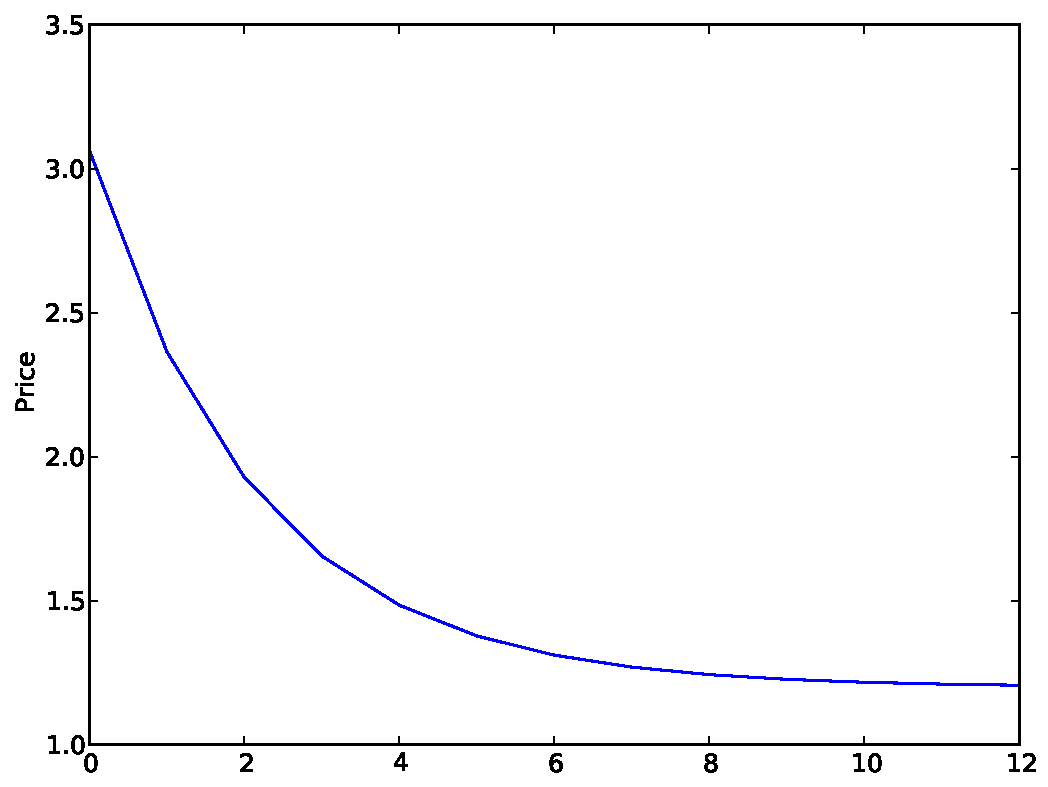
\includegraphics[scale=0.33]{conv_BC_price}
    \label{fig:conv_BC_price}
  } 
\subfloat[Regulator's tax]{
    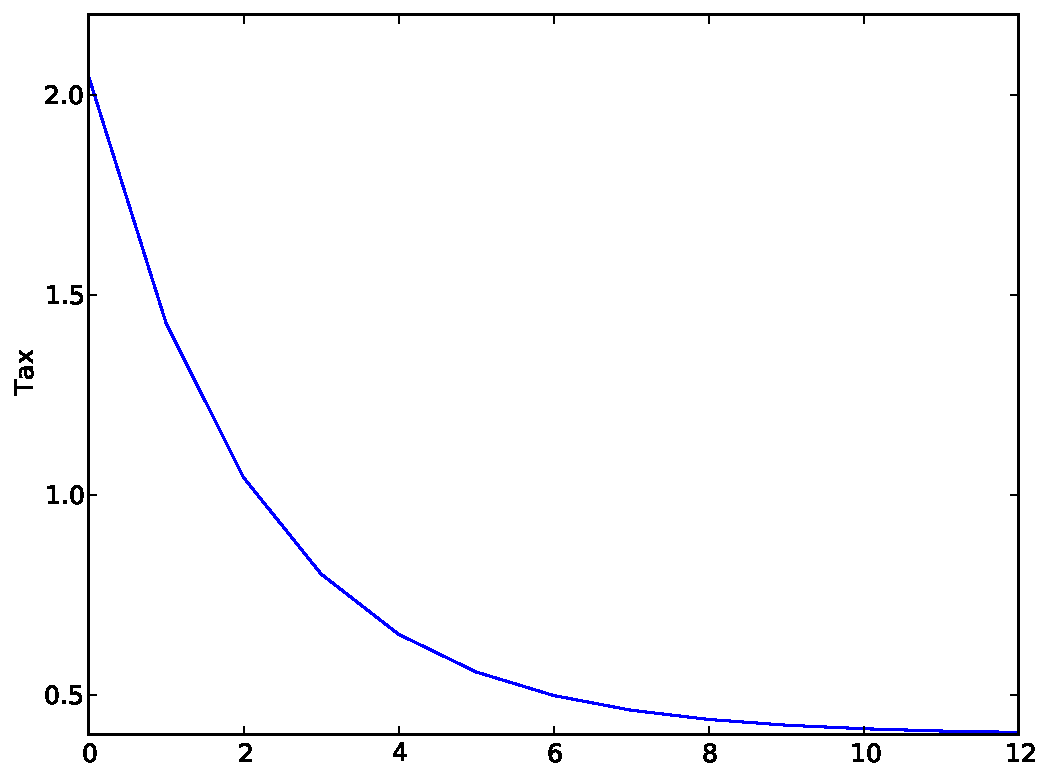
\includegraphics[scale=0.33]{conv_BC_tax}
    \label{fig:conv_BC_tax}
  }\newline
\subfloat[Demand]{
    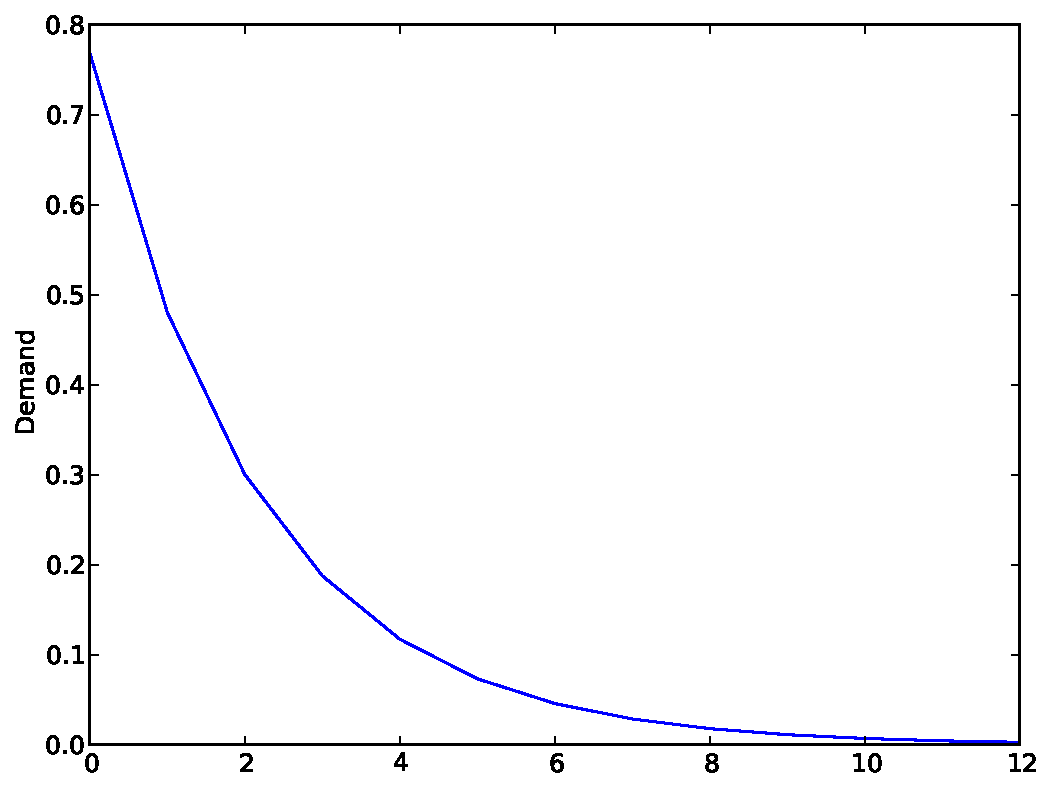
\includegraphics[scale=0.33]{conv_BC_demand}
    \label{fig:conv_BC_demand}
  } 
\subfloat[Monopolist's profit]{
    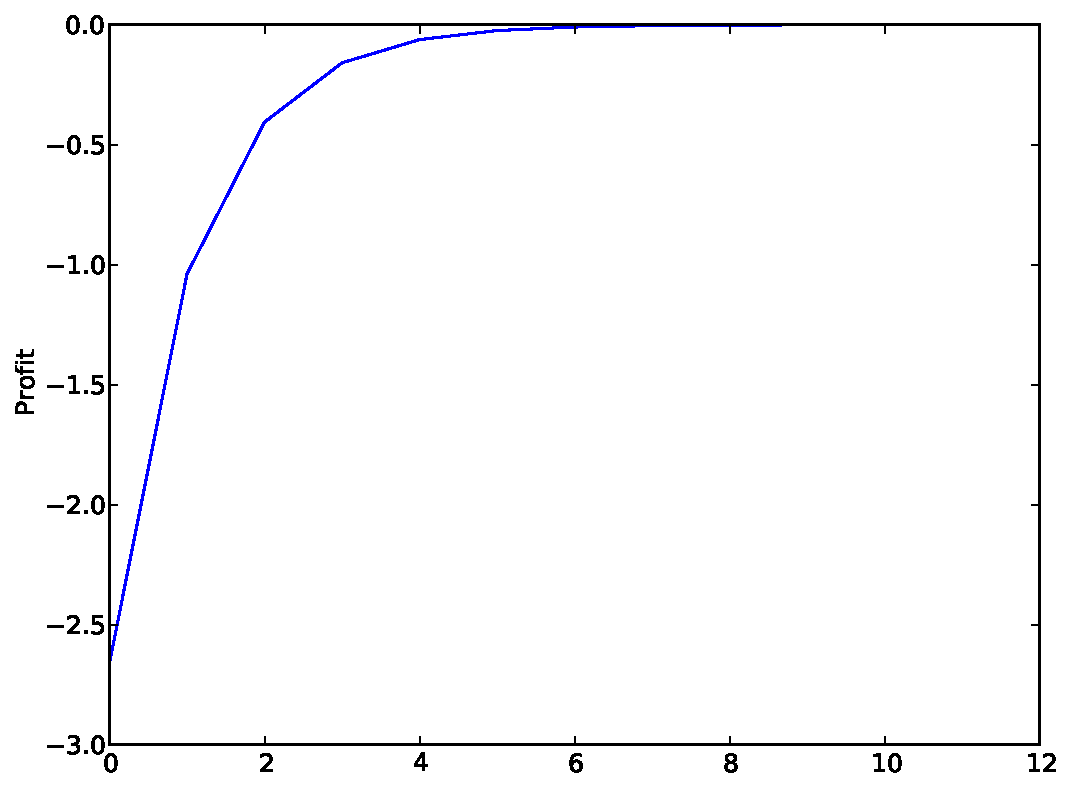
\includegraphics[scale=0.33]{conv_BC_profit}
    \label{fig:conv_BC_profit}
  }\newline
\subfloat[Pollution]{
    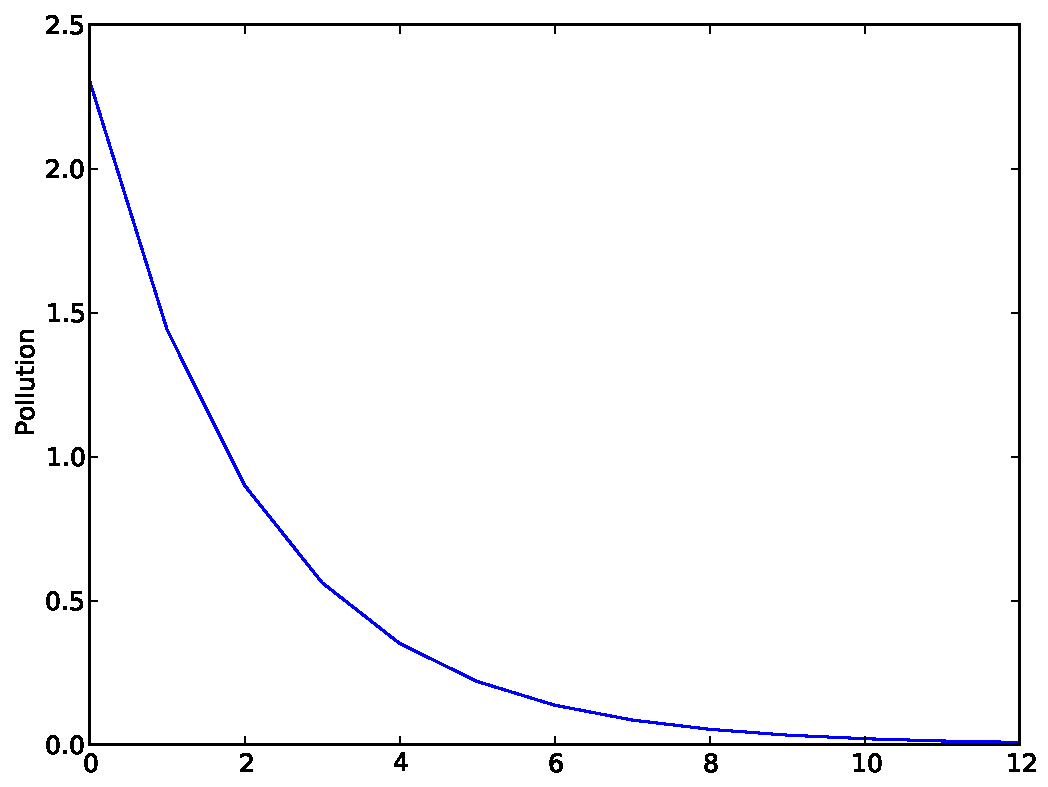
\includegraphics[scale=0.33]{conv_BC_pollution}
    \label{fig:conv_BC_pollution}
  } 
\subfloat[Welfare]{
    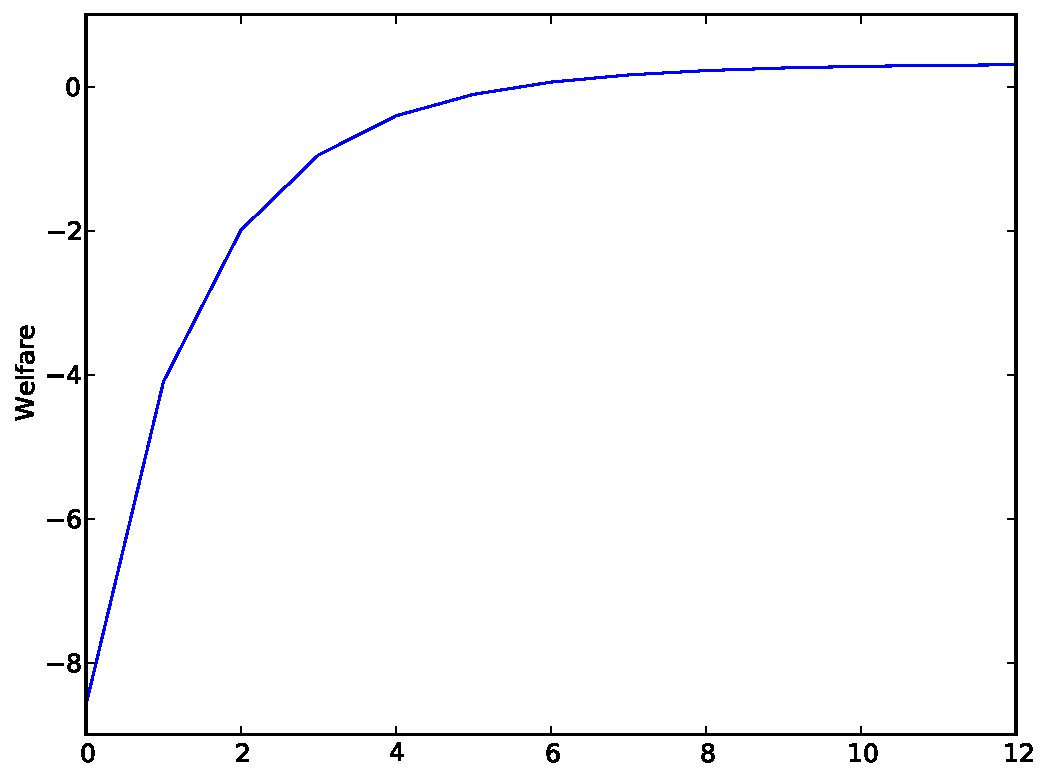
\includegraphics[scale=0.33]{conv_BC_welfare}
    \label{fig:conv_BC_welfare}
  }
\caption{Convergence in the base case over $12$ periods}
\label{fig:conv_BC_plots}
\end{figure}

The price is falling over time as the market participants with the greatest
valuation of the good purchase and exit the market. Therefore, condition %
\eqref{eq:1} is satisfied. The price gradually converges towards a steady
state of $\bar{p}\approx 1.2$ (see Appendix \ref{cha:numerical-results} for
a precise value). It should be noted that the steady state is an asymptote
of the price trajectory and is not reached in finite time.

Demand declines over time as the price differences across periods diminish.
If the price were to reach the steady state level, demand would drop to
zero. But since the steady state is approached only asymptotically, demand
is positive in all periods. As demand declines, so does the level of
pollution generated by production (Figure \ref{fig:conv_BC_pollution}).

Notably, firm profits are negative in this example. This raises the question
of why would this firm want to stay in business. Remember that the profits
reported in Figure \ref{fig:conv_BC_profit} are after-tax. Pre-tax profits
happen to be positive in all periods. As the monopolist cares about net
profits, the regulator could return the tax revenues to the monopolist as a
lump-sum transfer to keep him in business. Indeed, the point of taxation in
this model is to induce optimal behaviour, not to redistribute wealth. Thus,
there is nothing inherently objectionable about returning the revenues to
the monopolist. So long as the government's transfers to the monopolist are
not conditional on the current state variables, the efficiency of the
monopolist's decisions will not be affected.

Given our initial conditions, the equilibrium tax rate is also declining
over time as pollution levels are reduced. In the steady state the level of
taxation is about a third of the sale price ($\bar{\tau}\approx 0.4$). The
declining pollution externality reduces the need for taxation to alleviate
the problem. In addition, the monopolist's time inconsistency causes them to
charge a lower price in the current period in order to offset their
incentive for a price reduction in the following period. As prices in
consecutive periods converge over time, that incentive is reduced.
Consequently, the level of taxation required to correct for the monopolist's
inconsistency also declines.

The final variable charted in Figure \ref{fig:conv_BC_plots} is
instantaneous welfare. It is initially negative but converges to a positive
value as the pollution level drops. The positive value of the welfare is
driven by consumer surplus.

So far, the convergence paths of each variable in the base case accord with
what might be expected. Having canvassed them, we now turn to variations of
the parameters in Table \ref{tab:jmp_params} and the effect that such
variations have on the convergence paths and steady state levels of $\bar{p}$
and $\bar{\tau}$.

\section{Varying parameters}

\label{sec:varying-parameters-1}

Variation of the parameters is conducted in two parts. First, variations
that affect the convergence paths are considered. The simulation results
demonstrate that the parameters with the greatest impact upon convergence
paths are the time preference parameters, $\delta$ and $\beta$. The
remaining parameters have a negligible effect upon convergence rates: it
would not be visible at the scale plotted above in Figure \ref%
{fig:conv_BC_plots}. Consequently, convergence plots are given only for
those two variables.

The implications of the remaining variables for the equilibrium outcome are
analysed solely through their effect on the steady state levels $\bar{p}$
and $\bar{\tau}$.

\subsection{Convergence across parameter values}

\label{sec:conv-across-param}

In this subsection, the effect of varying the time preference parameters on
convergence rates is investigated.

\subsubsection{Varying $\protect\beta$}

\label{sec:varying-beta}

The first parameter that we vary is $\beta $, the consumer discount rate. It
embodies both the rate of consumer time preference and the depreciation rate
of the durable good. Consequently, it is rather lower than one might expect
for an ordinary time preference rate. In the base case, we set it to $\beta
=0.5$. For the variation we consider a range of values between $0.49$ and $%
0.52$. Beyond that range the steady state of the system is not in the
neighbourhood of the base case.

\begin{figure}[]
\centering
\subfloat[Monopolist's price]{
    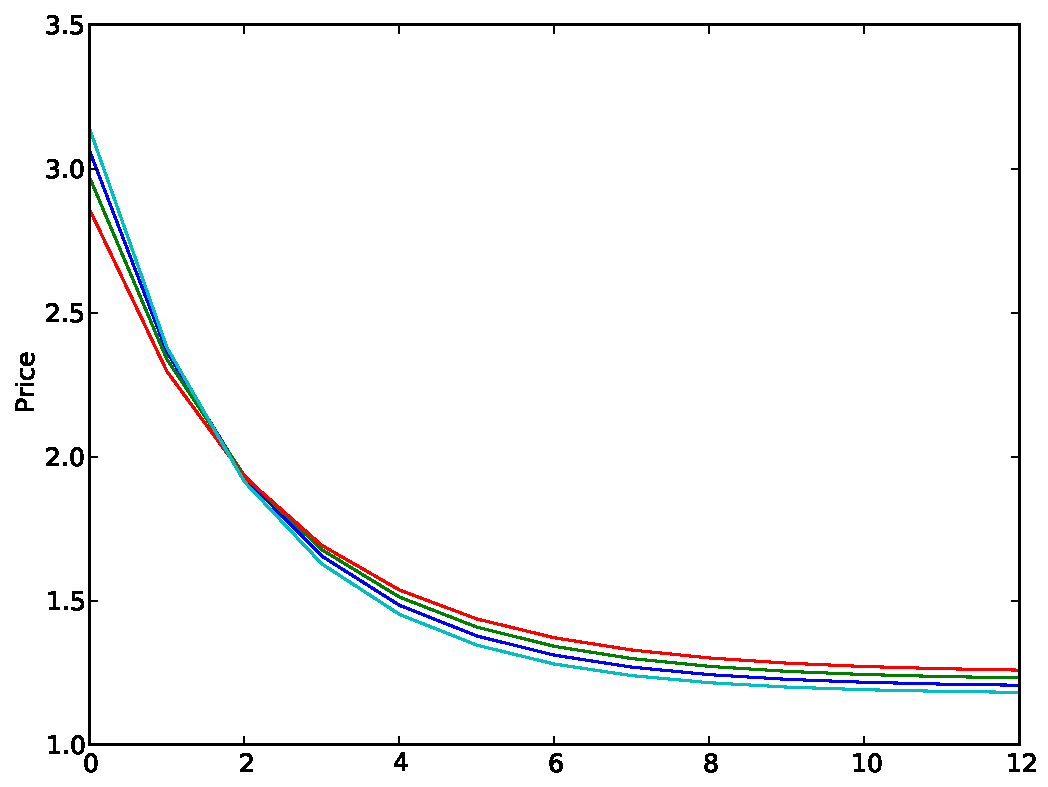
\includegraphics[scale=0.33]{conv_Beta_price}
    \label{fig:conv_Beta_price}
  } 
\subfloat[Regulator's tax]{
    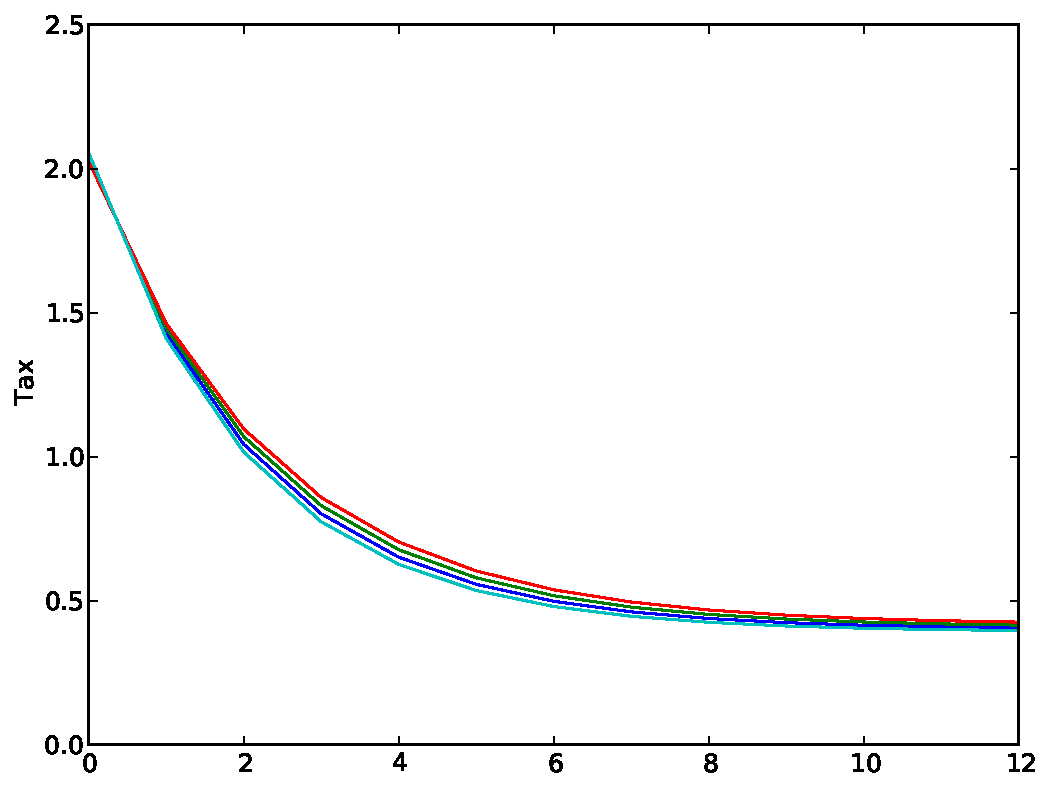
\includegraphics[scale=0.33]{conv_Beta_tax}
    \label{fig:conv_Beta_tax}
  }\newline
\subfloat[Demand]{
    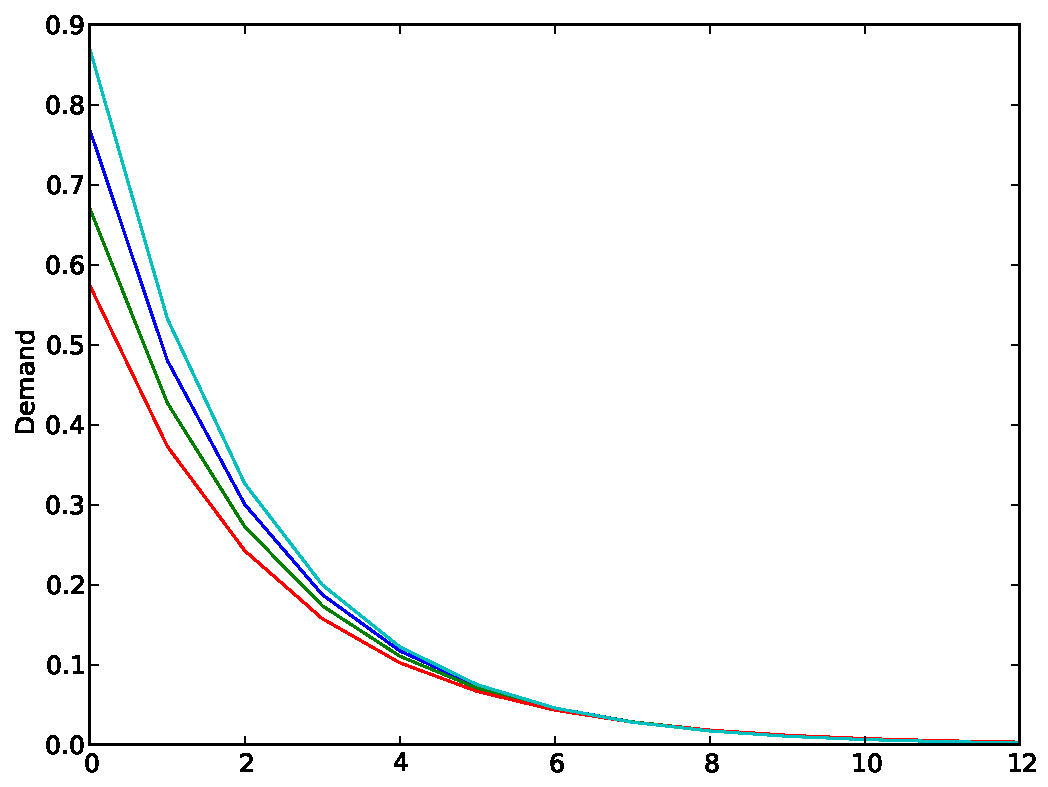
\includegraphics[scale=0.33]{conv_Beta_demand}
    \label{fig:conv_Beta_demand}
  } 
\subfloat[Monopolist's profit]{
    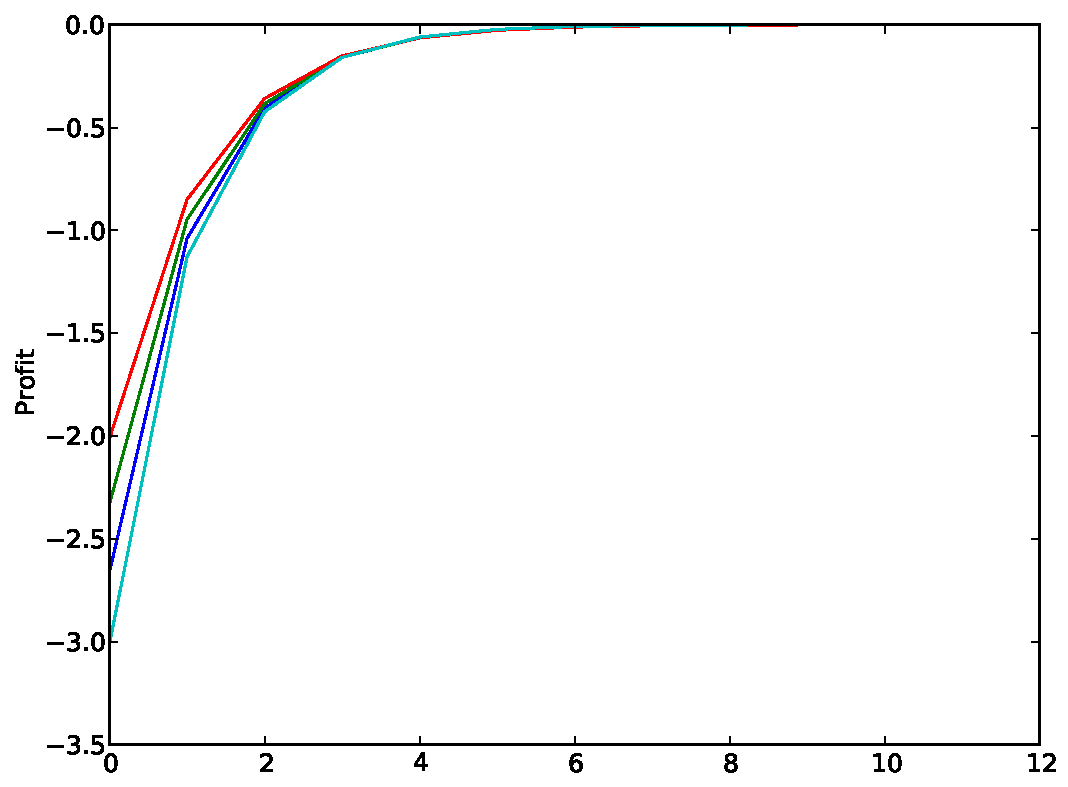
\includegraphics[scale=0.33]{conv_Beta_profit}
    \label{fig:conv_Beta_profit}
  }\newline
\subfloat[Pollution]{
    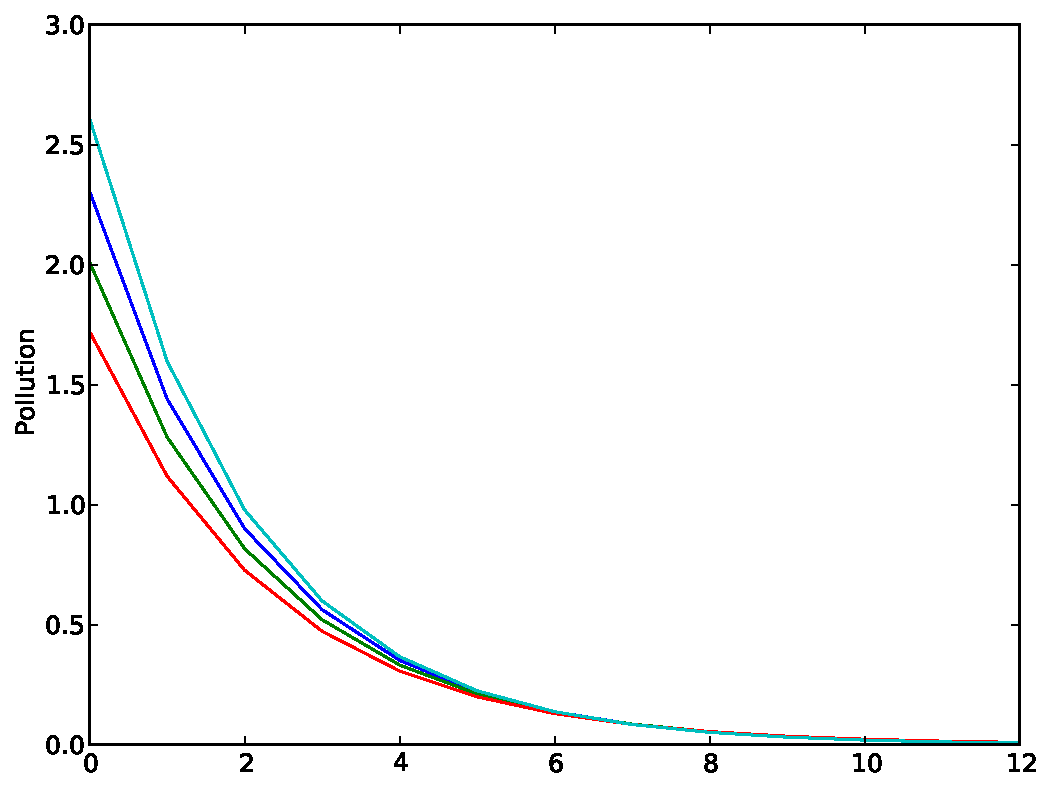
\includegraphics[scale=0.33]{conv_Beta_pollution}
    \label{fig:conv_Beta_pollution}
  } 
\subfloat[Welfare]{
    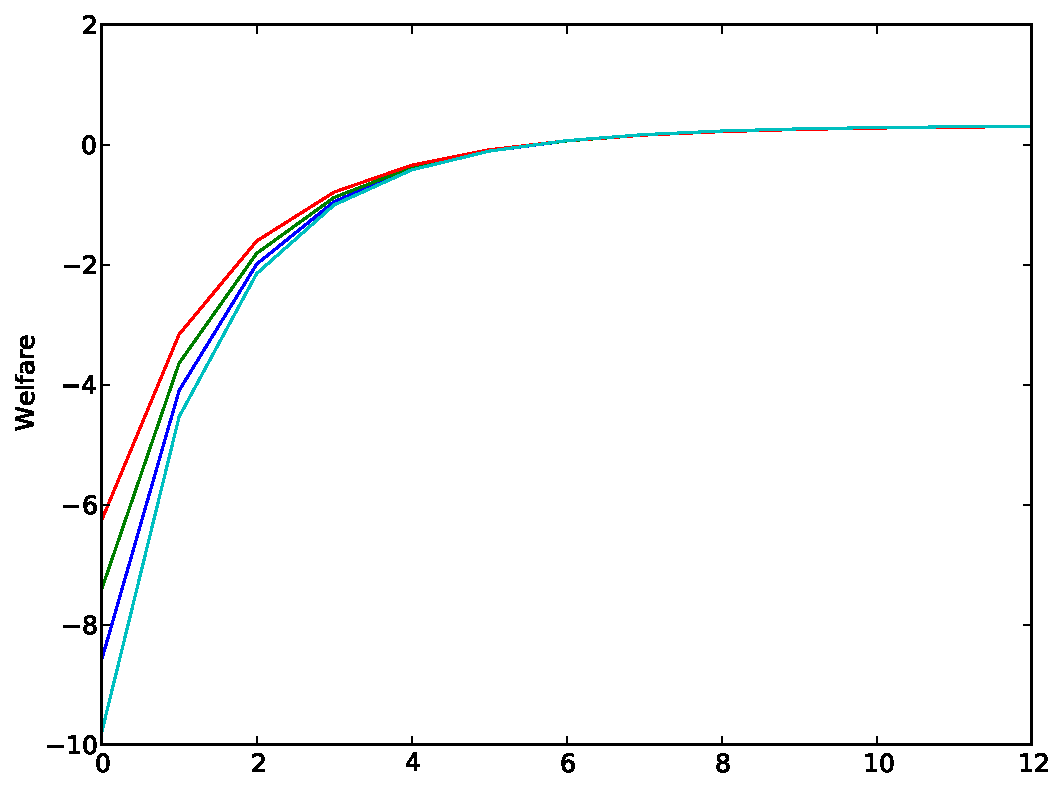
\includegraphics[scale=0.33]{conv_Beta_welfare}
    \label{fig:conv_Beta_welfare}
  }
\caption{Convergence for $\protect\beta \in \{0.49, 0.5, 0.51, 0.52\}$}
\label{fig:conv_beta_plots}
\end{figure}

The results are shown in Figure \ref{fig:conv_beta_plots} where $\beta =0.49$%
. The lower end of the range is denoted by the pale blue line and $\beta
=0.52$, at the upper end, is in red. The first thing to notice is that the
trajectory of demand is steeper when $\beta $ is lower. A lower value of $%
\beta $ decreases the value of postponing consumption, as the perceived
value of the durable good in the next period is lower. Consequently,
socially optimal consumption is shifted to earlier periods and demand is
initially higher but falls more quickly since there is a constant mass of
consumers. The increase in demand in early periods also pushes up pollution
levels and results in higher total pollution flows, which also cost the
monopolist profits due to the higher taxation. Interestingly, despite the
higher pollution levels the regulator chooses not to change the tax rate
significantly across the range of $\beta $'s tested.

\subsubsection{Varying $\protect\delta$}

\label{sec:varying-delta}

\begin{figure}[]
\centering
\subfloat[Monopolist's price]{
    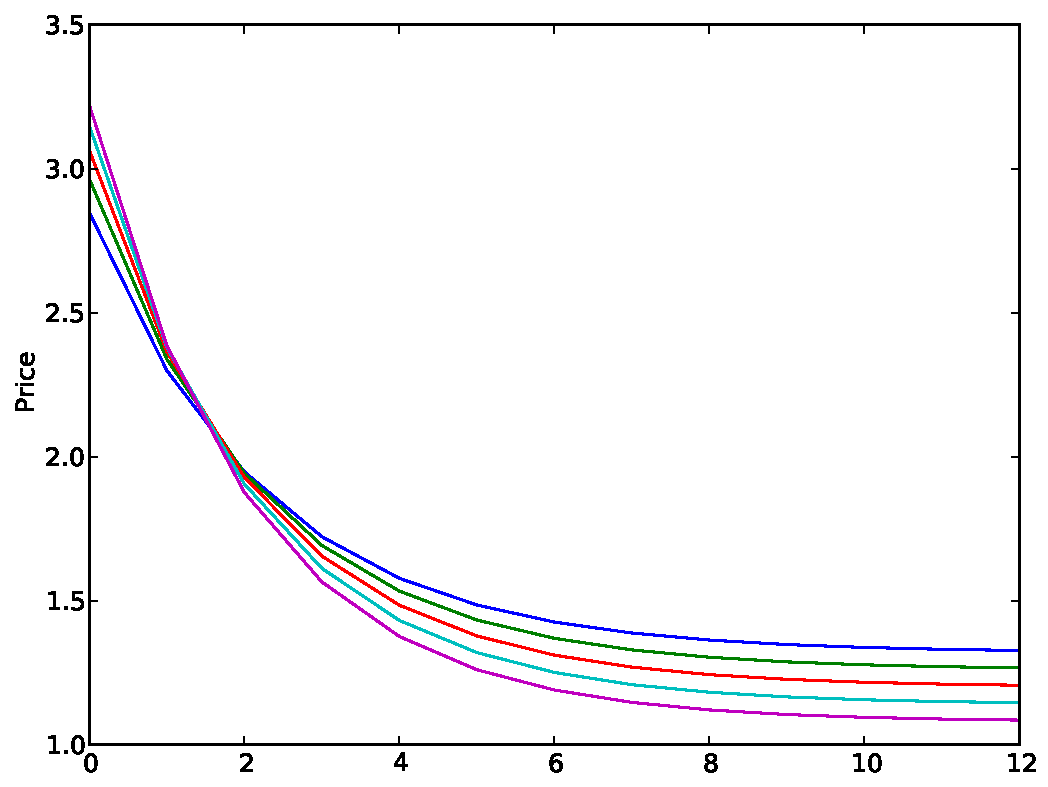
\includegraphics[scale=0.33]{conv_Delta_price}
    \label{fig:conv_Delta_price}
  } 
\subfloat[Regulator's tax]{
    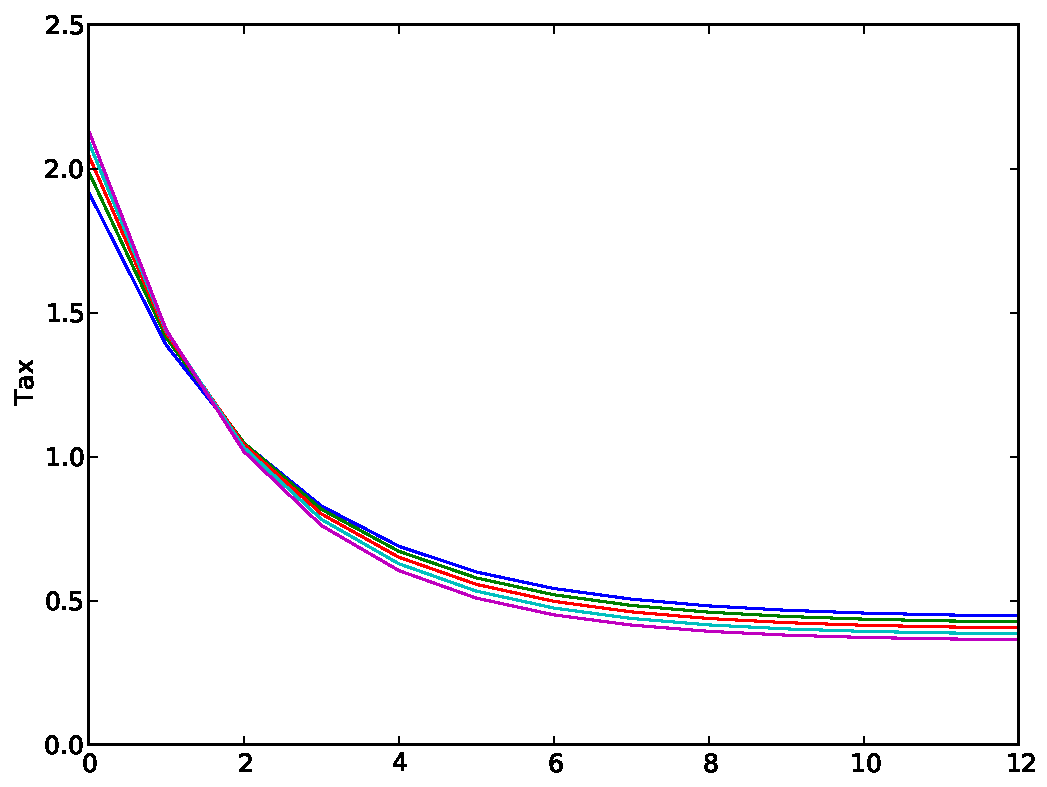
\includegraphics[scale=0.33]{conv_Delta_tax}
    \label{fig:conv_Delta_tax}
  }\newline
\subfloat[Demand]{
    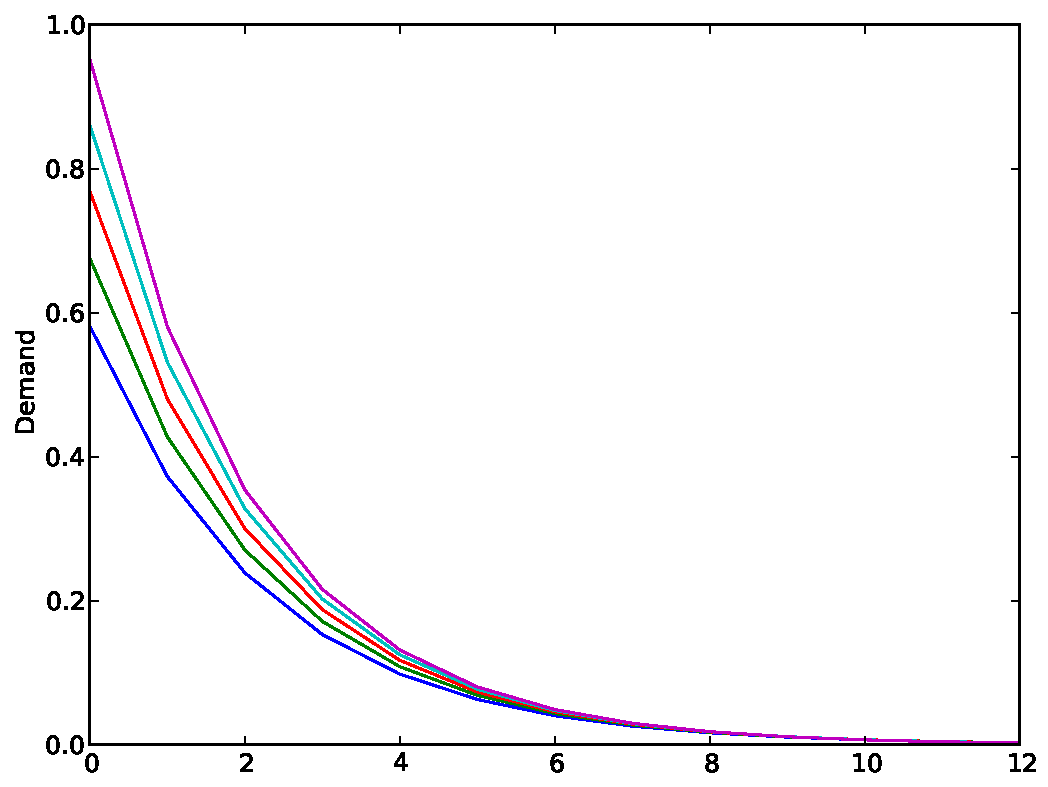
\includegraphics[scale=0.33]{conv_Delta_demand}
    \label{fig:conv_Delta_demand}
  } 
\subfloat[Monopolist's profit]{
    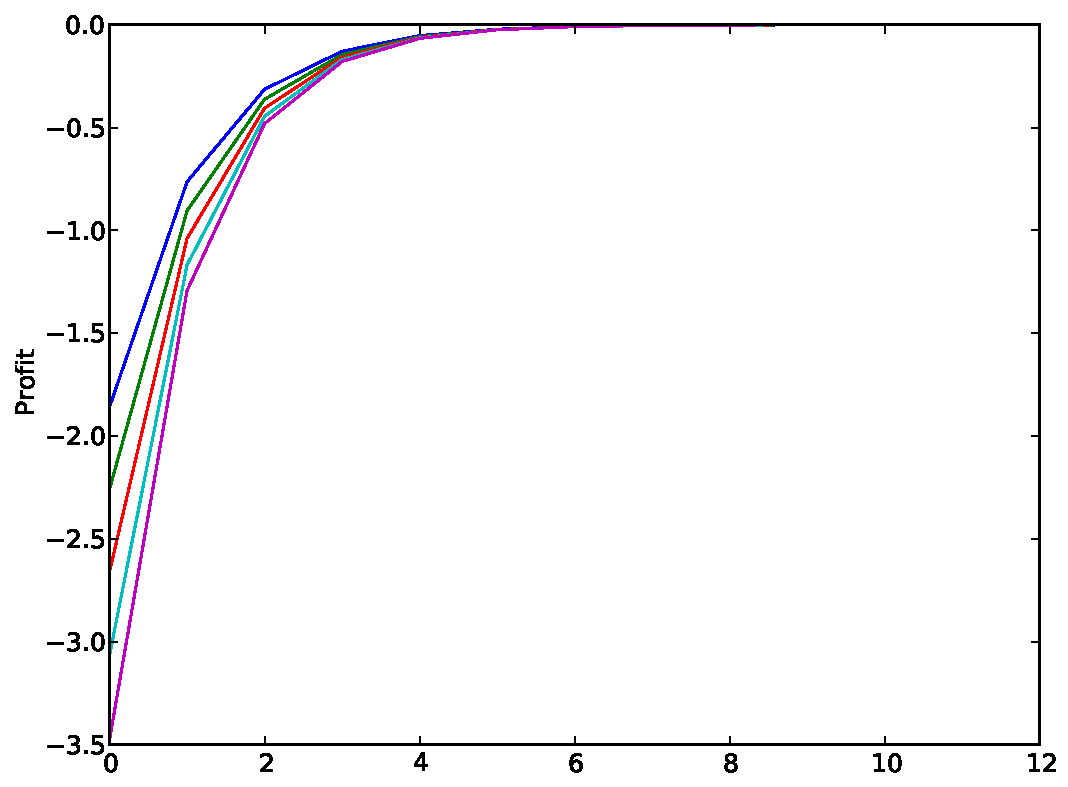
\includegraphics[scale=0.33]{conv_Delta_profit}
    \label{fig:conv_Delta_profit}
  }\newline
\subfloat[Pollution]{
    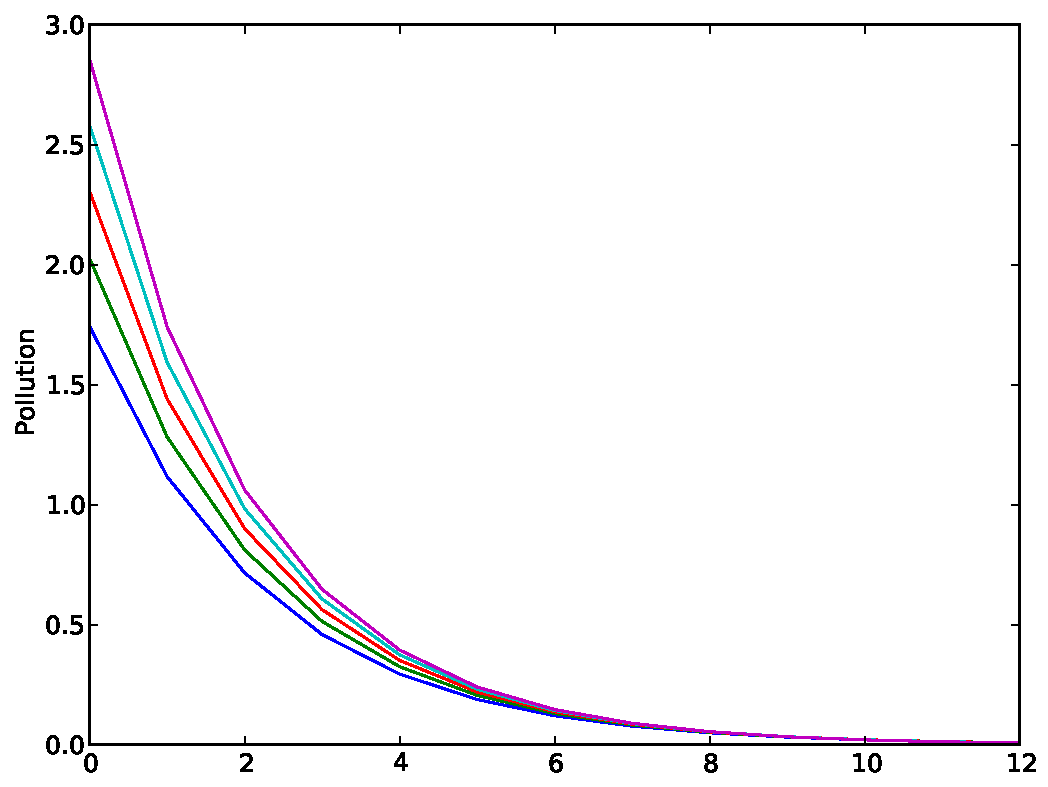
\includegraphics[scale=0.33]{conv_Delta_pollution}
    \label{fig:conv_Delta_pollution}
  } 
\subfloat[Welfare]{
    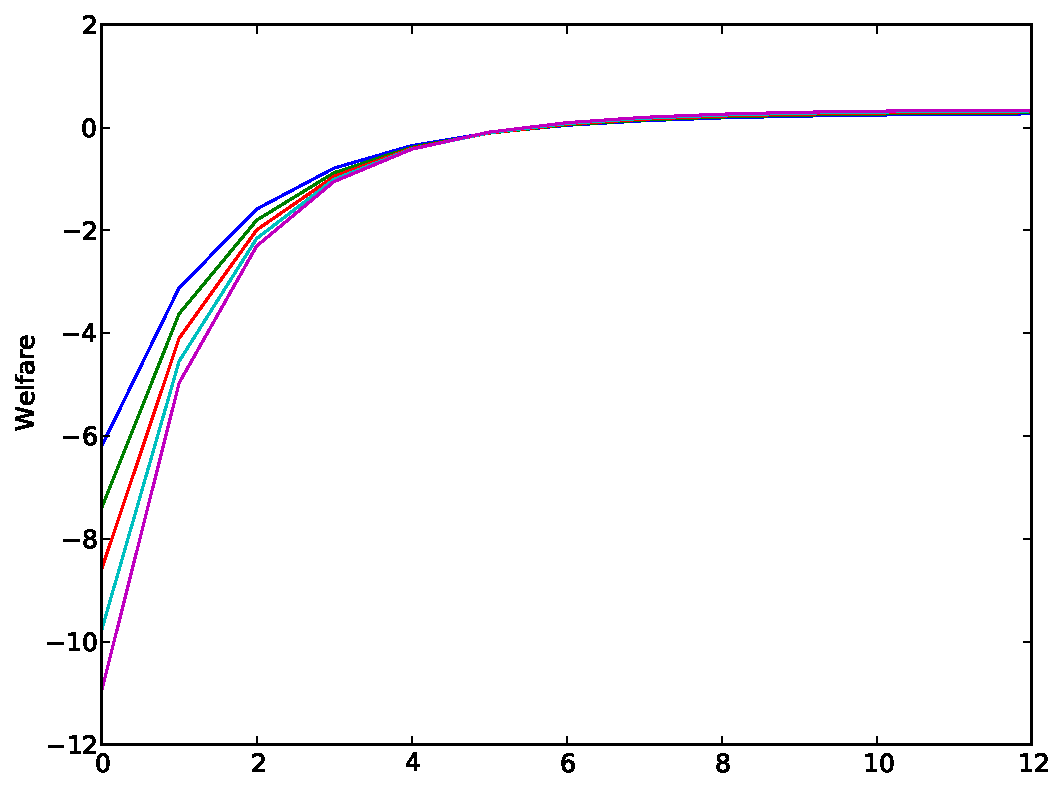
\includegraphics[scale=0.33]{conv_Delta_welfare}
    \label{fig:conv_Delta_welfare}
  }
\caption{Convergence for $\protect\delta \in \{0.78, 0.79, 0.8, 0.81, 0.82\}$
}
\label{fig:conv_delta_plots}
\end{figure}

The final part of our examination of convergence is an investigation of
variations of the discount factor of the government and the monopolist, $%
\delta $. It describes how future payoffs are valued relative to the current
period's payoff in the taxation game. The results are shown in Figure \ref%
{fig:conv_delta_plots} and are very similar to the results for variation in $%
\beta $, as one might expect for another time preference parameter.

The only notable differences are in the magnitude of the effect and the
impact upon the tax rate. The magnitude of the effect is slightly greater
since $\beta$ influences all future values, rather then solely consumers'
valuations of the durable good. However, it is the path of the tax rate that
is more interesting.

In Figure \ref{fig:conv_Beta_tax} the tax rate varied little between
different values of $\beta$ whereas, in Figure \ref{fig:conv_Delta_tax}, the
tax rate shows similar variation to the price path.

\subsection{Steady states across parameter values}

\label{sec:steady-states-across}

\begin{figure}[ht]
\centering
\subfloat[$\beta \in \{ 0.49, 0.5, 0.51, 0.52 \}$, $\delta \in \{
   0.78, 0.79, 0.8, 0.81, 0.82 \}$]{
    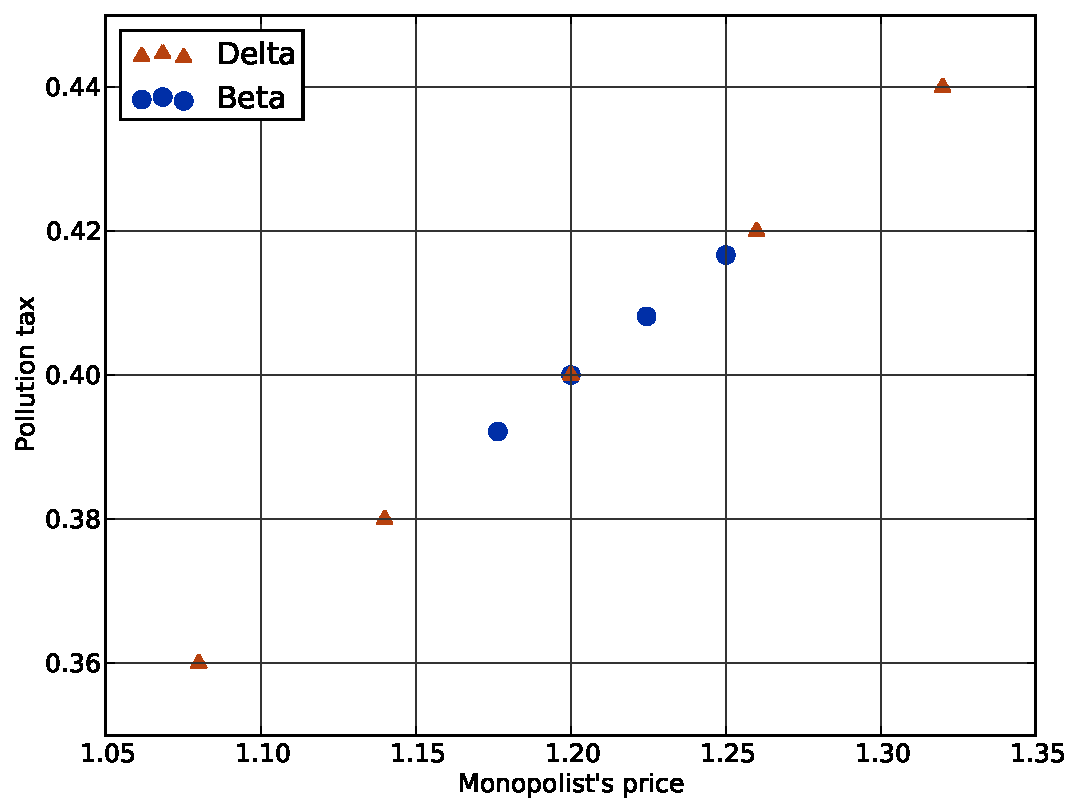
\includegraphics[scale=0.4]{SS_beta_delta}
    \label{fig:SS_beta_delta}
  }\newline
\subfloat[$\kappa \in \{ 2.98, 2.99, 3, 3.01, 3.02 \}$, $\alpha \in
   \{ 0.98, 0.99, 1 \}$]{
    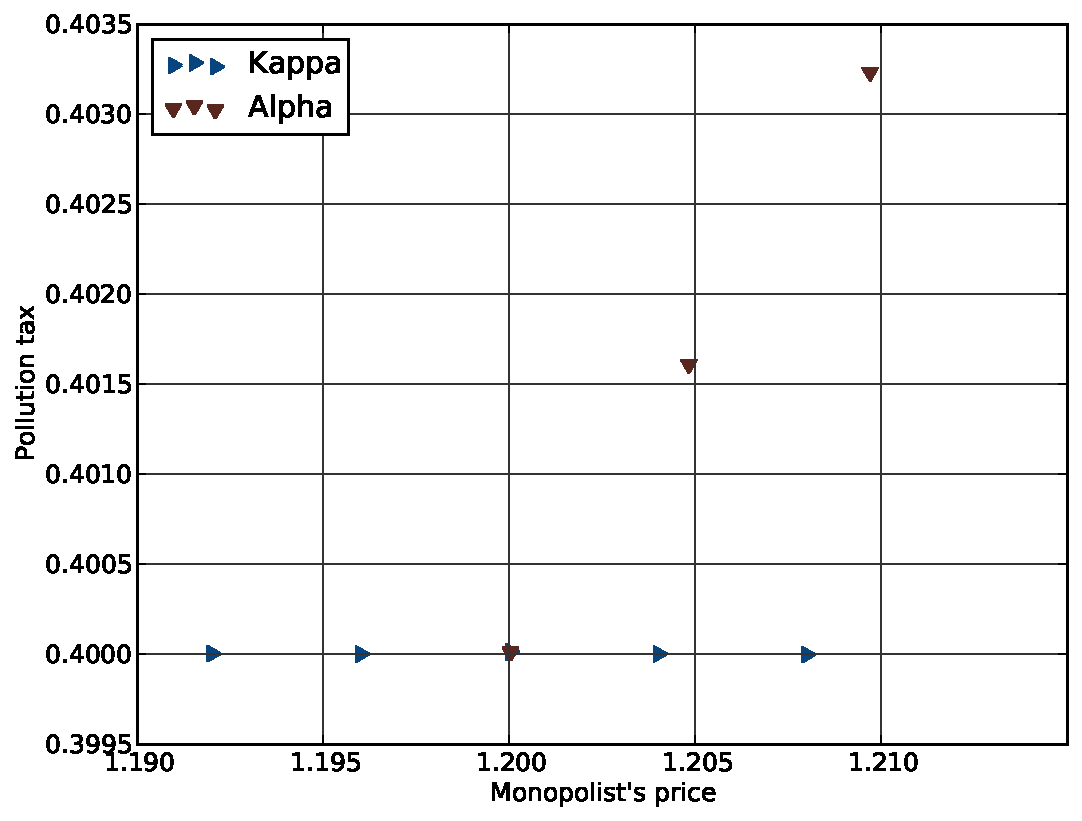
\includegraphics[scale=0.4]{SS_kappa_alpha}
    \label{fig:SS_kappa_alpha}
  }\newline
\subfloat[$\theta \in \{ 0, 0.01, 0.02 \}$, $\rho \in \{ 0.98,
   0.99, 1, 1.01, 1.02 \}$]{
    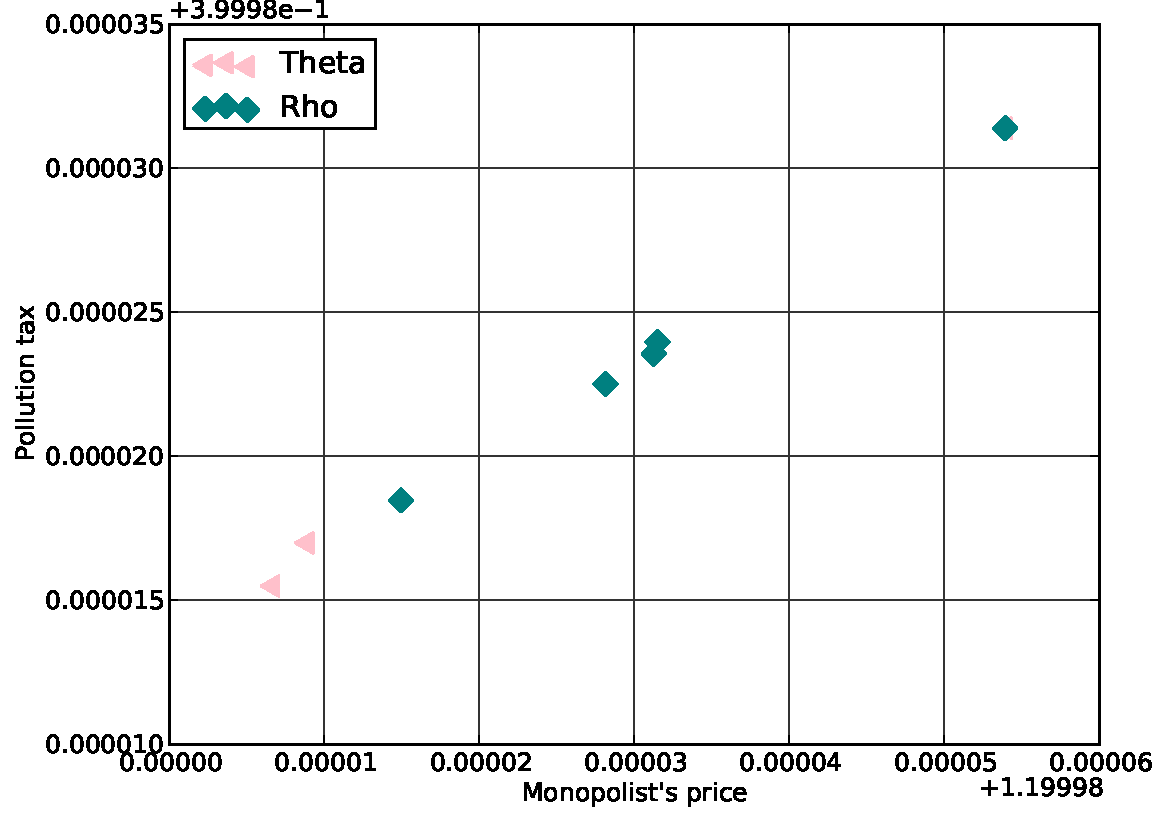
\includegraphics[scale=0.4]{SS_theta_rho}
    \label{fig:SS_theta_rho}
   }
\caption{Variation in steady states across parameter values}
\label{fig:ss_plots}
\end{figure}

Having examined the impact on convergence of time preference rates we now
turn to the steady state comparison. In this subsection we focus on the
difference in steady states as the parameters vary. Figure \ref{fig:ss_plots}
shows a scatter plot of $\bar{p}$ and $\bar{\tau}$ for pairs of parameter
values. The pairs are chosen by the magnitude of their effect so the scale
of the plot shrinks from Figure \ref{fig:SS_beta_delta} through to Figure %
\ref{fig:SS_theta_rho}.

A indicated in the previous section, the time preference rates have the
greatest impact on the result and in a similar fashion; $\delta$ with
greater magnitude than $\beta$. That is clearly shown by Figure \ref%
{fig:SS_beta_delta}, which indicates that the effect of each on the steady
state is identical in direction and varies only in magnitude. As agents
reduce their valuation of future payoffs the monopolist is forced to lift
their production and reduce their price in order to maintain demand for
their product. That, in turn generates pollution and causes a commensurate
lift in the tax rate to compensate.

In Figure \ref{fig:SS_kappa_alpha} the government's valuation of tax
revenues, $\alpha$, and the pollution function's coefficient, $\kappa$, are
varied. The effect of a drop in $\alpha$ is to increase the tax rate levied
by the regulator while changing the rate of pollution has no effect upon the
tax rate but does affect the price charged by the monopolist.

Finally, Figure \ref{fig:SS_theta_rho} shows the negligible impact that the
cost of policy changes, $\theta$, and the production cost coefficient, $\rho$%
, have on the steady state. Increasing $\rho$ causes the monopolist to
increase prices, as might be expected when their marginal costs rise;
however, the scale of the impact is such that it is an insignificant effect
relative to that of time preference and the coefficient on pollution.

%%% Local Variables:
%%% mode: latex
%%% TeX-master: "root"
%%% End:
